%%%%%%%%%%%%%%%%%%%%%%%%%%%%%%%%%%%%%%%%%%%%%%%%%%%%%%%%%%%%%%%%%%%%%%%%%%%%%%%
% PLANTILLA DE WHITE PAPER TÉCNICO - WASAFF CONSULTING
% VERSIÓN 11.1 (CORREGIDA Y OPTIMIZADA)
% ESTRUCTURA BASADA EN EVIDENCIA CUANTITATIVA Y CONSECUENCIAS DE NEGOCIO
%%%%%%%%%%%%%%%%%%%%%%%%%%%%%%%%%%%%%%%%%%%%%%%%%%%%%%%%%%%%%%%%%%%%%%%%%%%%%%%

\documentclass[11pt, a4paper,oneside]{article}

%=============== PREÁMBULO: CONFIGURACIÓN DEL DOCUMENTO =======================

\usepackage[utf8]{inputenc}
\usepackage[spanish, es-tabla]{babel}
\usepackage{graphicx}
\usepackage{geometry}
\usepackage{xcolor}
\usepackage{fancyhdr}
\usepackage{titlesec}
\usepackage{booktabs}
\usepackage{hyperref}
\usepackage[most]{tcolorbox}
\usepackage{parskip}

% --- MEJORA 10/10: PAQUETE DE MICRO-TIPOGRAFÍA PROFESIONAL ---
\usepackage{microtype} %%% <--- AÑADIDO: Mejora el espaciado y justificación del texto

% --- Geometría y Colores ---
% --- CORREGIDO: Aumentamos el headheight para que calce el encabezado ---
\geometry{a4paper, left=2.5cm, right=2.5cm, top=2.5cm, bottom=2.5cm, headheight=38pt} %%% <--- CORREGIDO
\definecolor{WasaffNavy}{HTML}{001F3F}
\definecolor{WasaffCopper}{HTML}{B87333}
\definecolor{LightGray}{HTML}{F5F5F5}

% --- Fuentes y Títulos ---
\usepackage{lmodern} 
\usepackage{tgheros} 
\renewcommand*\familydefault{\sfdefault}
\titleformat{\section}
  {\normalfont\Large\bfseries\color{WasaffNavy}}
  {\thesection.}{1em}{}
\titleformat{\subsection}
  {\normalfont\large\bfseries\color{WasaffCopper}}
  {\thesubsection.}{1em}{}
\renewcommand*\familydefault{\rmdefault} 

% --- Encabezado y Pie de Página ---
\pagestyle{fancy}
\fancyhf{}
\fancyhead[L]{
\includegraphics[height=1cm]{wasaff_logo.png}}
\fancyhead[R]{\color{gray}\fontsize{9}{11}\selectfont \begin{tabular}{r} WHITE PAPER TÉCNICO \\ \textit{De la Aproximación a la Certeza Física} \end{tabular}}
\fancyfoot[C]{\color{gray}\thepage}
\renewcommand{\headrulewidth}{0.4pt}

% --- Configuración de Hyperref ---
\hypersetup{
    colorlinks=true, linkcolor=WasaffNavy, urlcolor=WasaffCopper,
    pdftitle={Análisis Cuantitativo: Simulación CFD vs. Cálculos Empíricos en Diseño de Tuberías},
    pdfauthor={Felipe Wasaff - Wasaff Consulting},
    pdfsubject={Un análisis comparativo basado en primeros principios para la toma de decisiones.}
}

% --- Cajas de texto personalizadas ---
\tcbuselibrary{skins}
\newtcolorbox{abstractbox}{
    enhanced, colback=LightGray, colframe=WasaffNavy, fonttitle=\bfseries, arc=1mm, boxrule=0.5pt,
    title={Resumen Ejecutivo (Abstract)}, top=3mm, bottom=3mm
}
\newtcolorbox{resultbox}[2][]{
    enhanced, colback=#2!5, colframe=#2, fonttitle=\bfseries, arc=1mm, boxrule=1pt,
    title=#1, top=4mm, bottom=4mm, halign title=center
}
\newtcolorbox{ctabox}{
    enhanced, colback=WasaffNavy!10, colframe=WasaffCopper, fonttitle=\bfseries, arc=1mm, boxrule=1pt,
    title={De la Incertidumbre a la Decisión Inteligente}, top=4mm, bottom=4mm
}

%=============== DOCUMENTO PRINCIPAL =========================================
\begin{document}
\sffamily

% --- BLOQUE DEL TÍTULO ---
\
\vspace{1cm}
{\color{WasaffCopper} \large \textbf{WHITE PAPER TÉCNICO}}\\
\
{\color{WasaffNavy} \huge \textbf{El Manifold de Enfriamiento de 5 Millones de Dólares}}\\
\
{\Large Un Caso Práctico: Cómo un Diseño Basado en Suposiciones Pone en Riesgo el Rendimiento de una Inversión Crítica}\\
\
\vspace{1cm}
\
\rmfamily
\begin{tabular}{@{}p{14cm}}
    \textbf{Autor:} Felipe Wasaff \\
    \textit{Fundador, Wasaff Consulting} \\
    \href{mailto:felipe@wasaffconsulting.com}{felipe@wasaffconsulting.com} \\
\end{tabular}
\vspace{1cm}

\begin{abstractbox}
    Este informe técnico demuestra, a través de un caso práctico, los riesgos de negocio inherentes a diseñar componentes de fluidos críticos, como manifolds de distribución, basándose en cálculos empíricos y suposiciones de simetría. Analizamos un manifold de enfriamiento para una línea de producción valorada en 5 millones de dólares, comparando el diseño por aproximación (que predice una distribución de flujo uniforme) con la realidad revelada por la Simulación CFD (que muestra una severa mala distribución). Cuantificamos la desviación numérica y la traducimos en consecuencias directas: sobrecalentamiento de activos, menor vida útil, cuellos de botella en la producción y un ROI fallido. Este documento concluye que el análisis basado en los primeros principios físicos no es un costo, sino una póliza de seguro indispensable para garantizar el rendimiento de inversiones de capital significativas.
\end{abstractbox}

\section{El Escenario: El Manifold de Enfriamiento Crítico}
Imagine esta situación: su empresa está invirtiendo 5 millones de dólares en una nueva línea de producción con cinco equipos idénticos. El éxito de toda la inversión depende de que cada equipo reciba un caudal de agua de enfriamiento equitativo desde un manifold de distribución. El equipo de ingeniería debe decidir entre usar cálculos manuales, asumiendo una distribución simétrica para entregar el diseño en dos días, o invertir en un análisis de simulación para garantizar el rendimiento. Este White Paper demuestra cómo estas dos decisiones llevan a dos futuros de negocio radicalmente diferentes.

\section{El Camino de la ``Experiencia'': El Diseño por Aproximación Empírica}
El método estándar se basa en una suposición fundamental: que un manifold geométricamente simétrico producirá una distribución de flujo simétrica.

\begin{figure}[h!]
    \centering
    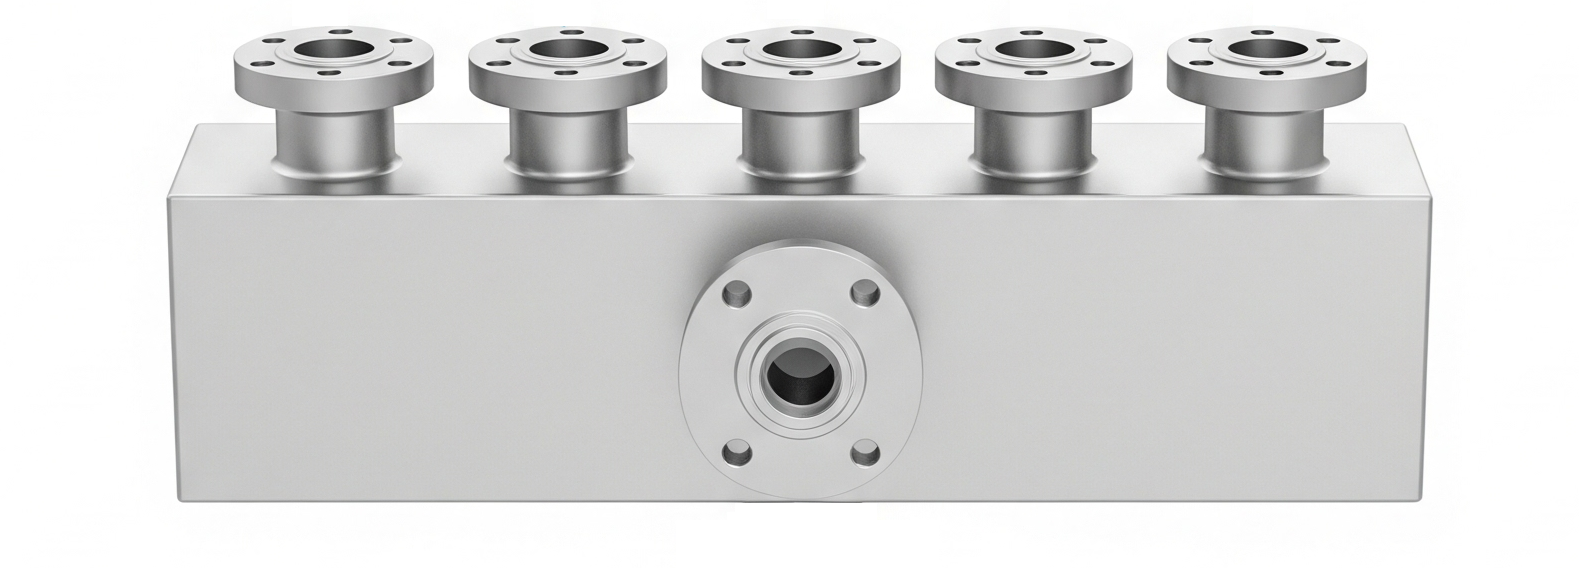
\includegraphics[width=0.7\textwidth]{manifold_diseno_empirico.png}
    \caption{Ilustración del diseño del manifold basado en la suposición de simetría. Se asume que cada una de las 5 salidas recibirá un 20\% del flujo total.}
    \label{fig:empirico}
\end{figure}

Basado en esta premisa, la conclusión del cálculo es que el diseño es viable, prediciendo una caída de presión ($\Delta P$) de \textbf{[0.35 bar]} y una distribución de flujo de **20\%** a cada salida.

\section{El Camino de la Física: La Realidad Revelada por la Simulación}
No asumimos nada. Aplicamos las leyes de Navier-Stokes directamente sobre la geometría 3D. El resultado revela una cruda realidad física que la intuición y los promedios no pueden predecir.

\begin{figure}[h!]
    \centering
  %  \includegraphics[width=0.9\textwidth]{manifold_realidad_cfd.png}
    \caption{Resultado de la simulación CFD. Se observa cómo el momento del fluido privilegia a las primeras salidas, dejando a las últimas con un flujo deficiente.}
    \label{fig:cfd}
\end{figure}

El análisis físico real predice:
\begin{itemize}
    \item Caída de Presión Real ($\Delta P$): \textbf{[0.48 bar]} (Un \textbf{[37\%]} mayor que la predicción empírica).
    \item Distribución de Flujo Real:
        \begin{itemize}
            \item Equipo 1: \textbf{[28\%]}
            \item Equipo 2: \textbf{[23\%]}
            \item Equipo 3: \textbf{[19\%]}
            \item Equipo 4: \textbf{[16\%]}
            \item Equipo 5: \textbf{[14\%]} --- ¡Recibe apenas la mitad que el primero!
        \end{itemize}
\end{itemize}

\section{La Decisión del Gerente: Una Tabla de Consecuencias de Negocio}
La "experiencia" nos habría llevado a aprobar un diseño inherentemente defectuoso. La diferencia entre asumir y calcular se traduce directamente en los siguientes riesgos y costos para la inversión de 5 millones de dólares:

\begin{table}[h!]
    \centering
    \caption{Impacto en el negocio de un diseño basado en suposiciones vs. física.}
    \label{tab:consecuencias}
    \begin{tabular}{p{3.5cm} p{6cm} p{6cm}}
    \toprule
    \textbf{Consecuencia} & \textbf{Impacto del Diseño Empírico} & \textbf{Beneficio del Análisis Físico} \\
    \midrule
    \textbf{Rendimiento de Activos} & El equipo 5 opera sobrecalentado, reduciendo su vida útil en un 40\%. El equipo 1 opera demasiado frío, afectando la calidad. & Cada activo opera en su punto óptimo, **maximizando la vida útil y la consistencia de la producción**. \\
    \addlinespace
    \textbf{Mantenimiento} & Fallas no programadas en el equipo 5, requiriendo detenciones de toda la línea de producción. & Mantenimiento predecible y menor tasa de fallas. **Reducción del costo de mantenimiento reactivo**. \\
    \addlinespace
    \textbf{Producción y ROI} & La línea nunca alcanza su capacidad de diseño. Se crea un cuello de botella que **invalida el ROI del proyecto**. & La línea es fiable y alcanza su capacidad nominal. **Se asegura y protege el retorno de la inversión de 5 MUSD.** \\
    \addlinespace
    \textbf{Eficiencia Energética} & La bomba (seleccionada con $\Delta P$ subestimado) trabaja forzada, **consumiendo un 20\% más de energía**. & La bomba correcta es seleccionada, operando en su punto de máxima eficiencia. **Se asegura el menor OPEX posible**. \\
    \bottomrule
    \end{tabular}
\end{table}

\begin{ctabox}
    Como demuestra este escenario, el costo de un análisis físico profundo es insignificante comparado con el costo de operar con un diseño basado en suposiciones.
    
    Mi servicio de \textbf{Diagnóstico Estratégico de 10 Días} está diseñado para responder a estas preguntas críticas en la etapa de diseño, \textit{antes} de que se cometan errores de millones de dólares. No es una simulación; es una póliza de seguro para el rendimiento de su inversión.
    
    \
    \centering
    \href{https://www.wasaffconsulting.com/como-empezar}{\color{WasaffCopper} \large \textbf{ASEGURE EL ROI DE SU PROYECTO - AGENDAR MI DIAGNÓSTICO}}
\end{ctabox}

\vspace{2cm}
---
\
{\small
\textbf{Sobre el autor:} Felipe Wasaff es Físico y Técnico en Automatización, fundador de Wasaff Consulting. Se especializa en aplicar la simulación computacional y los primeros principios para garantizar el rendimiento de inversiones de capital en la industria.
}

\end{document} 